%
%  analysis_report
%
%  Created by Sam Cook on 2012-11-06.
%  Copyright (c) 2012 . All rights reserved.
%
\documentclass[]{article}

% Use utf-8 encoding for foreign characters
\usepackage[utf8]{inputenc}

% Setup for fullpage use
\usepackage{fullpage}

% Uncomment some of the following if you use the features
%
% Running Headers and footers
%\usepackage{fancyhdr}

% Multipart figures
%\usepackage{subfigure}

% More symbols
\usepackage{amsmath}
%\usepackage{amssymb}
%\usepackage{latexsym}

% Surround parts of graphics with box
\usepackage{boxedminipage}

% Package for including code in the document
\usepackage{listings}

% If you want to generate a toc for each chapter (use with book)
\usepackage{minitoc}

% This is now the recommended way for checking for PDFLaTeX:
\usepackage{ifpdf}

%\newif\ifpdf
%\ifx\pdfoutput\undefined
%\pdffalse % we are not running PDFLaTeX
%\else
%\pdfoutput=1 % we are running PDFLaTeX
%\pdftrue
%\fi

\newcommand{\nth}[1]{$#1^\text{th}$}
\newcommand{\nthTwo}[2]{$#1^\text{#2}$}
\newcommand{\ms}{$\mu$s}

\ifpdf
\usepackage[pdftex]{graphicx}
\else
\usepackage{graphicx}
\fi
\title{MuSIC 5 Analsis Report}
\author{Sam Cook}

\date{2012-11-06}

\begin{document}

\ifpdf
\DeclareGraphicsExtensions{.pdf, .jpg, .tif}
\else
\DeclareGraphicsExtensions{.eps, .jpg}
\fi

\maketitle


\begin{abstract}
	The \nth{5} MuSIC beam-time (\nth{18} to the \nthTwo{22}{nd} June 2012) was intended to test the momentum distribution of the muons beam. Here we will discuss the strategy employed to analyse the data and the problems encountered.
\end{abstract}

\section{Introduction} % (fold)
\label{sec:introduction}
The analysis of the \nth{5}~MuSIC beam time splits into 5~logical sub-algorithms called here: `Run Data' (Section~\ref{sec:run_data}), `Simulated Data' (Section~\ref{sec:simulated_data}), `Acceptance' (Section~\ref{sec:acceptance}), `Fitting and Integration' (Section~\ref{sec:fitting_and_integration}) and `Muon Yield' (Section~\ref{sec:muon_yield}). The `Run' and `Simulated Data' algorithms cover the processing of the initial data to such a point as they can be treated identically. The `Acceptance' section covers the calculation of the detector acceptance based on simulated data. The `Fitting and Integration' and `Muon Yield' sections cover the final stages of the algorithm in calculating the number of muon decays and ultimately the muon yield of the run. The overall flow can be seen in Figure~\ref{fig:analysis_flow_diagrm}.
\begin{figure}[htbp]
	\centering
		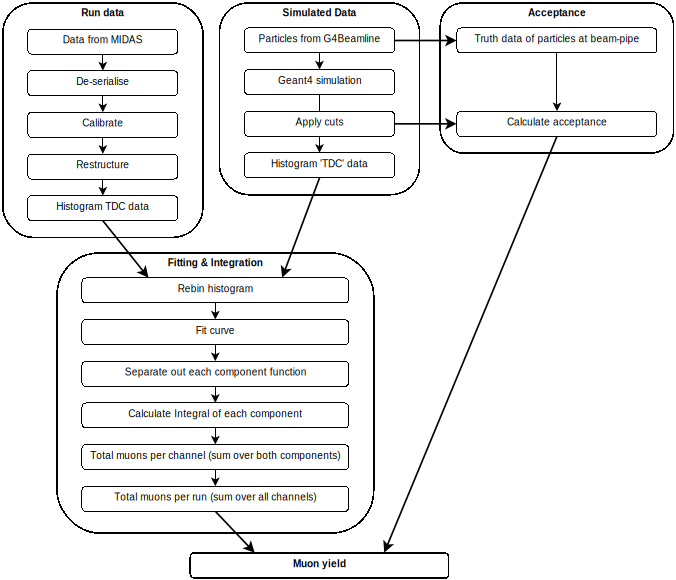
\includegraphics[width=\textwidth]{image/Analysis_flow_diagram.png}
	\caption{Flow diagram of the analysis' logic}
	\label{fig:analysis_flow_diagrm}
\end{figure}

% section introduction (end)
%%%%%%%%%%%%%%%%%%%%%%%%%%%%%%%%%%%%%%%%%%%%%%%%%%%%%%%%%%%%%%%%%%%%%%%%%%%%%%
\section{Experimental Set Up} % (fold)
\label{sec:experimental_set_up}

% section experimental_set_up (end)
%%%%%%%%%%%%%%%%%%%%%%%%%%%%%%%%%%%%%%%%%%%%%%%%%%%%%%%%%%%%%%%%%%%%%%%%%%%%%%
\section{Run Data} % (fold)
\label{sec:run_data}
As figure~\ref{fig:analysis_flow_diagrm} shows there are 5 main stages in preparing the real data for analysis. These will will be explained in more detail in the following sub-sections but the general process will be discussed here. The first stage is the receipt of data from the data acquisition system (DAQ) via MIDAS, this creates files of raw data which has to be (in some cases) de-serialised in the next stage before having calibration applied to it. The final stages are to restructure the data according to channel and then create histograms of the TDC values ready for analysis. 

These processes are split across 3 programs: MIDAS; mu\_analysis and mid2root\_converter (which act on .root and .mid MIDAS files respectively); and finally tdc\_file.py which is a python script for creating the TDC histograms.

% section run_data (end)
%%%%%%%%%%%%%%%%%%%%%%%%%%%%%%%%%%%%%%%%%%%%%%%%%%%%%%%%%%%%%%%%%%%%%%%%%%%%%%
\section{Simulated Data} % (fold)
\label{sec:simulated_data}

% section simulated_data (end)
%%%%%%%%%%%%%%%%%%%%%%%%%%%%%%%%%%%%%%%%%%%%%%%%%%%%%%%%%%%%%%%%%%%%%%%%%%%%%%
\section{Acceptance} % (fold)
\label{sec:acceptance}

% section acceptance (end)
%%%%%%%%%%%%%%%%%%%%%%%%%%%%%%%%%%%%%%%%%%%%%%%%%%%%%%%%%%%%%%%%%%%%%%%%%%%%%%
\section{Fitting And Integration} % (fold)
\label{sec:fitting_and_integration}

% section fitting_and_integration (end)
%%%%%%%%%%%%%%%%%%%%%%%%%%%%%%%%%%%%%%%%%%%%%%%%%%%%%%%%%%%%%%%%%%%%%%%%%%%%%%
\section{Muon Yield} % (fold)
\label{sec:muon_yield}

% section muon_yield (end)
%%%%%%%%%%%%%%%%%%%%%%%%%%%%%%%%%%%%%%%%%%%%%%%%%%%%%%%%%%%%%%%%%%%%%%%%%%%%%%
\bibliographystyle{plain}
\bibliography{}
\end{document}
